
\documentclass[refman]{article}
\usepackage[utf8]{inputenc}
\usepackage[english]{babel}


%

\usepackage{colortbl}
\usepackage{epigraph}
\usepackage{fancyhdr}
\usepackage{graphicx}
\usepackage{hhline}
%\usepackage{biblatex}
\usepackage{wrapfig}

\usepackage[procnames]{listings}
\usepackage{longtable}
\usepackage{tikz}
\usepackage{subcaption}
\usepackage{xcolor}
\usepackage{wrapfig}
\usepackage[nottoc,numbib]{tocbibind}
%
%\usepackage[T1]{fontenc}
\usepackage{lmodern}

\usepackage{amsfonts}
\usepackage{amsmath}
\usepackage{amsthm}
\usepackage{mathtools}

\usepackage{geometry}
 \geometry{
 a4paper,
 left=30mm,
 top=30mm,
 }
\pagestyle{fancy}

\newcommand{\idx}{\text{idx}}

\DeclarePairedDelimiter\ceil{\lceil}{\rceil}
\DeclarePairedDelimiter\floor{\lfloor}{\rfloor}

\theoremstyle{definition}
\newtheorem*{formula}{Formula}

\usepackage[document]{ragged2e}

\begin{document}

\begin{titlepage}
	\centering
	
\includegraphics[width=0.15\textwidth]{graphics/huberlin_logo}\par\vspace{1cm}
	{\scshape\LARGE Humboldt University of Berlin \par}
	\vspace{1cm}
	{\scshape\Large Projektpraktikum \par}
	\vspace{1.5cm}
	{\huge\bfseries Solving a Poisson's Equation Numerically \par}
	\vspace{2cm}
	{\Large\itshape Christian Parpart \& Kei Thoma \par}
	\vfill

	\vfill

% Bottom of the page
	{\large \today\par}
\end{titlepage}

\tableofcontents

\section{Introduction}

Previously \cite{protocol}, we discussed the numerical approach to the Poisson's equation. In essence, if we denote the dimension with \(d\), then the domain \(\Omega := [0, 1]^d\) is discretized into \(N^d\) points and the problem is reduced to a linear equation that is

\begin{align*}
	A^{(d)} u = b
\end{align*}

where \(A^{(d)}\) is the matrix which has a sparse structure and was defined in the last protocol. We will now explore numerical methods to solve the linear equation above.

For this, consider the function

\begin{align*}
	u(x) := \prod_{l=1}^d x_l \sin (\kappa \pi x_l)
\end{align*}

and since the Poisson's equation we want to solve is the following

\begin{align*}
	f(x) = - \Delta u(x) = -\sum_{l = 1}^d \frac{\partial^2 u}{\partial x_l^2} (x)
\end{align*}

we have

\begin{align*}
	f_{d=1} (x_1) =& \kappa \pi \left( \kappa \pi x_1 \sin ( \kappa \pi x ) - 2 \cos( \kappa \pi x_1) \right) \\
%	
	f_{d=2} (x_1, x_2) =& \kappa \pi x_2 \sin( \kappa \pi x_2) \left(  \kappa \pi x_1 \sin(\kappa \pi x_1) - 2 \cos ( \kappa \pi x_1) \right) + \\ 
	& \kappa \pi x_1 \sin( \kappa \pi x_1) \left(  \kappa \pi x_2 \sin(\kappa \pi x_2) - 2 \cos ( \kappa \pi x_2) \right) \\
%
	f_{d=3} (x_1, x_2, x_3) =& \kappa \pi x_2 \sin( \kappa \pi x_2) \kappa \pi x_3 \sin(\kappa \pi x_3)  \left(  \kappa \pi x_1 \sin(\kappa \pi x_1) - 2 \cos ( \kappa \pi x_1) \right) + \\
	& \kappa \pi x_1 \sin( \kappa \pi x_1) \kappa \pi x_3 \sin(\kappa \pi x_3)  \left(  \kappa \pi x_2 \sin(\kappa \pi x_2) - 2 \cos ( \kappa \pi x_2) \right) + \\
	& \kappa \pi x_1 \sin( \kappa \pi x_1) \kappa \pi x_2 \sin(\kappa \pi x_2)  \left(  \kappa \pi x_3 \sin(\kappa \pi x_3) - 2 \cos ( \kappa \pi x_3) \right) \text{.}
\end{align*}

We want to now solve the given linear equation for \(u\) (we will denote the numerical solution with \(\hat{u}\)) for each dimension and compare it with the original \(u\). To do this, we first apply the LU-decomposition to \(A^{(d)}\) and multiply the inverse of \(L\) and \(U\) with \(b\) to get \(b\).

\section{User Manual}

All result of this protocol can be recreated with the accompanying Python module. In the main function of this module, one may change the max_n variable to extend the presented plot.

\section{Error and Condition}

\begin{figure}[h]
	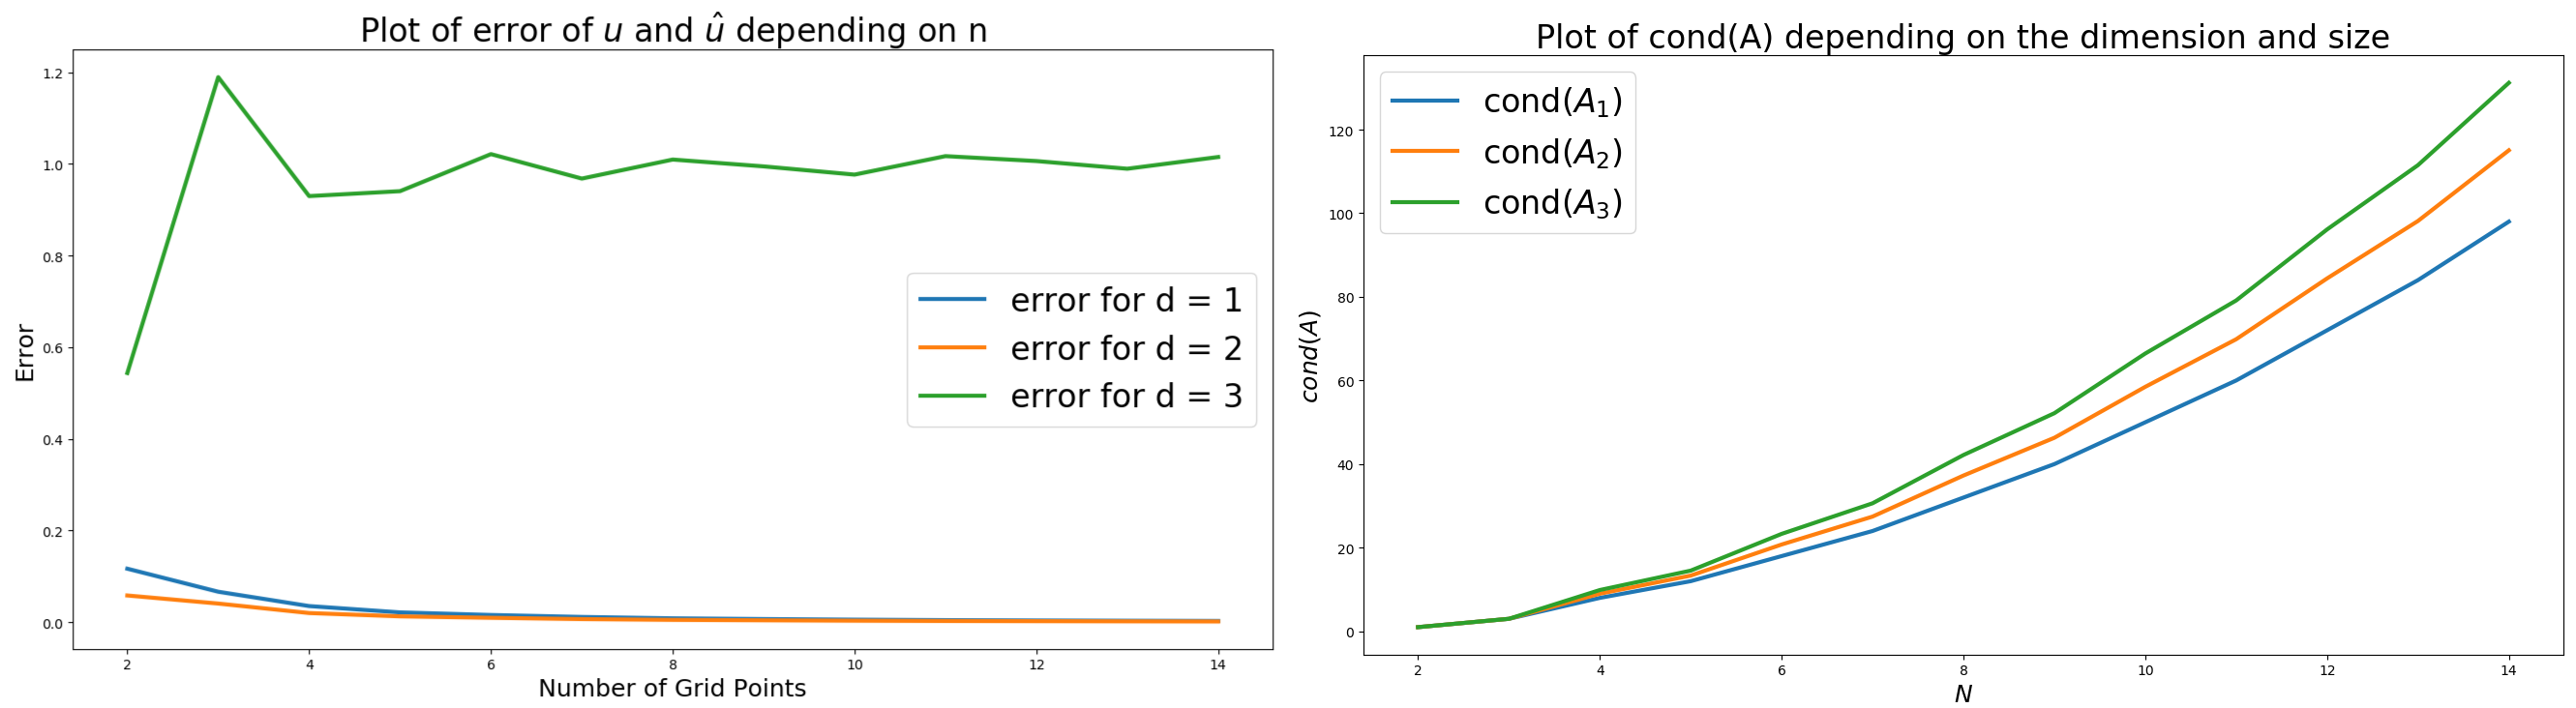
\includegraphics[width=\linewidth]{graphics/error_condition.png}
	\caption{Plot of the Error and the Condition of the Matrix}
	\label{fig:plot_error}
\end{figure}

We have drawn the plot of the absolute difference of \(u\) and \(\hat{u}\) for \(d = 1, 2, 3\) with the number of grid points on an axis \(N\) as the variable (see figure \ref{fig:plot_error}).

It turns out that the absolute error converges to a relativly small number. This is counter-intuitive at first because the condition number of the matrix \(A^{(d)}\) increases drastically for large \(N\) as seen on figure \ref{fig:plot_error}.

\begin{wrapfigure}{hr}{0.67\textwidth}
	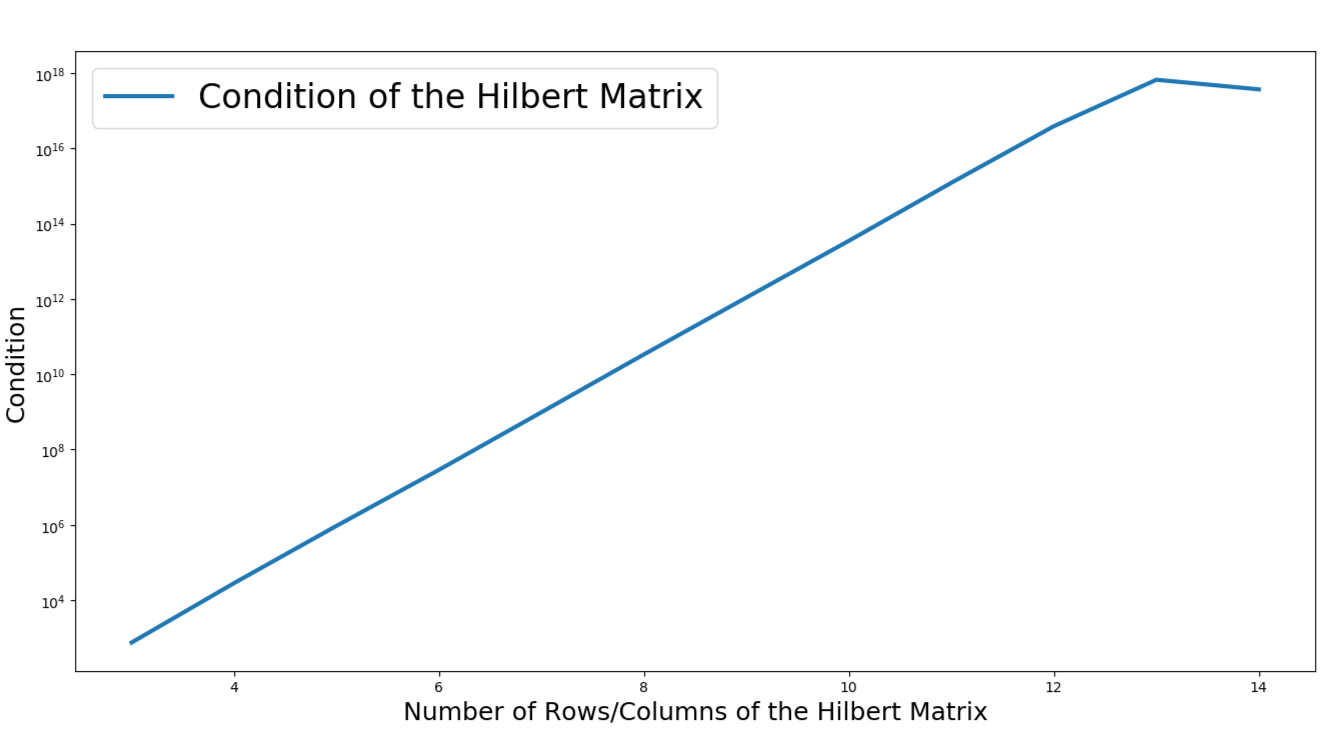
\includegraphics[width=0.65\textwidth]{graphics/hilbert_condition.png}
	\caption{Condition of the Hilbert Matrix}
	\label{fig:hilbert_condition}
\end{wrapfigure}

Why does the error of \(u\) and \(\hat{u}\) converge while the condition of \(A^{(d)}\) increases? To answer this question, we compare our results with the condition of the Hilbert Matrix which is well-known to be ill-conditioned (see figure \ref{fig:hilbert_condition}).

As one can see, the condition of the Hilbert matrix is so large that the condition of \(A^{(d)}\) pales in comparison. In other words, \(A^{(d)}\) is not as ill-conditioned as one might assume at first. Furthermore, intuitively, the increase in number of grid points should make the approximation of the solution to the Poission's equation more accurate which is reflected on the convergence of the error plots.

Figure \ref{fig:plots} illustrates this point. Here, we have plotted the analytical and the approximated solutions for the Poisson's equation for dimension 2 with different numbers of grid points (\(N = 4\) and \(N = 30\)). As the number of grid points increases the approximation becomes better verifying our statements above.

\begin{figure}[h]
	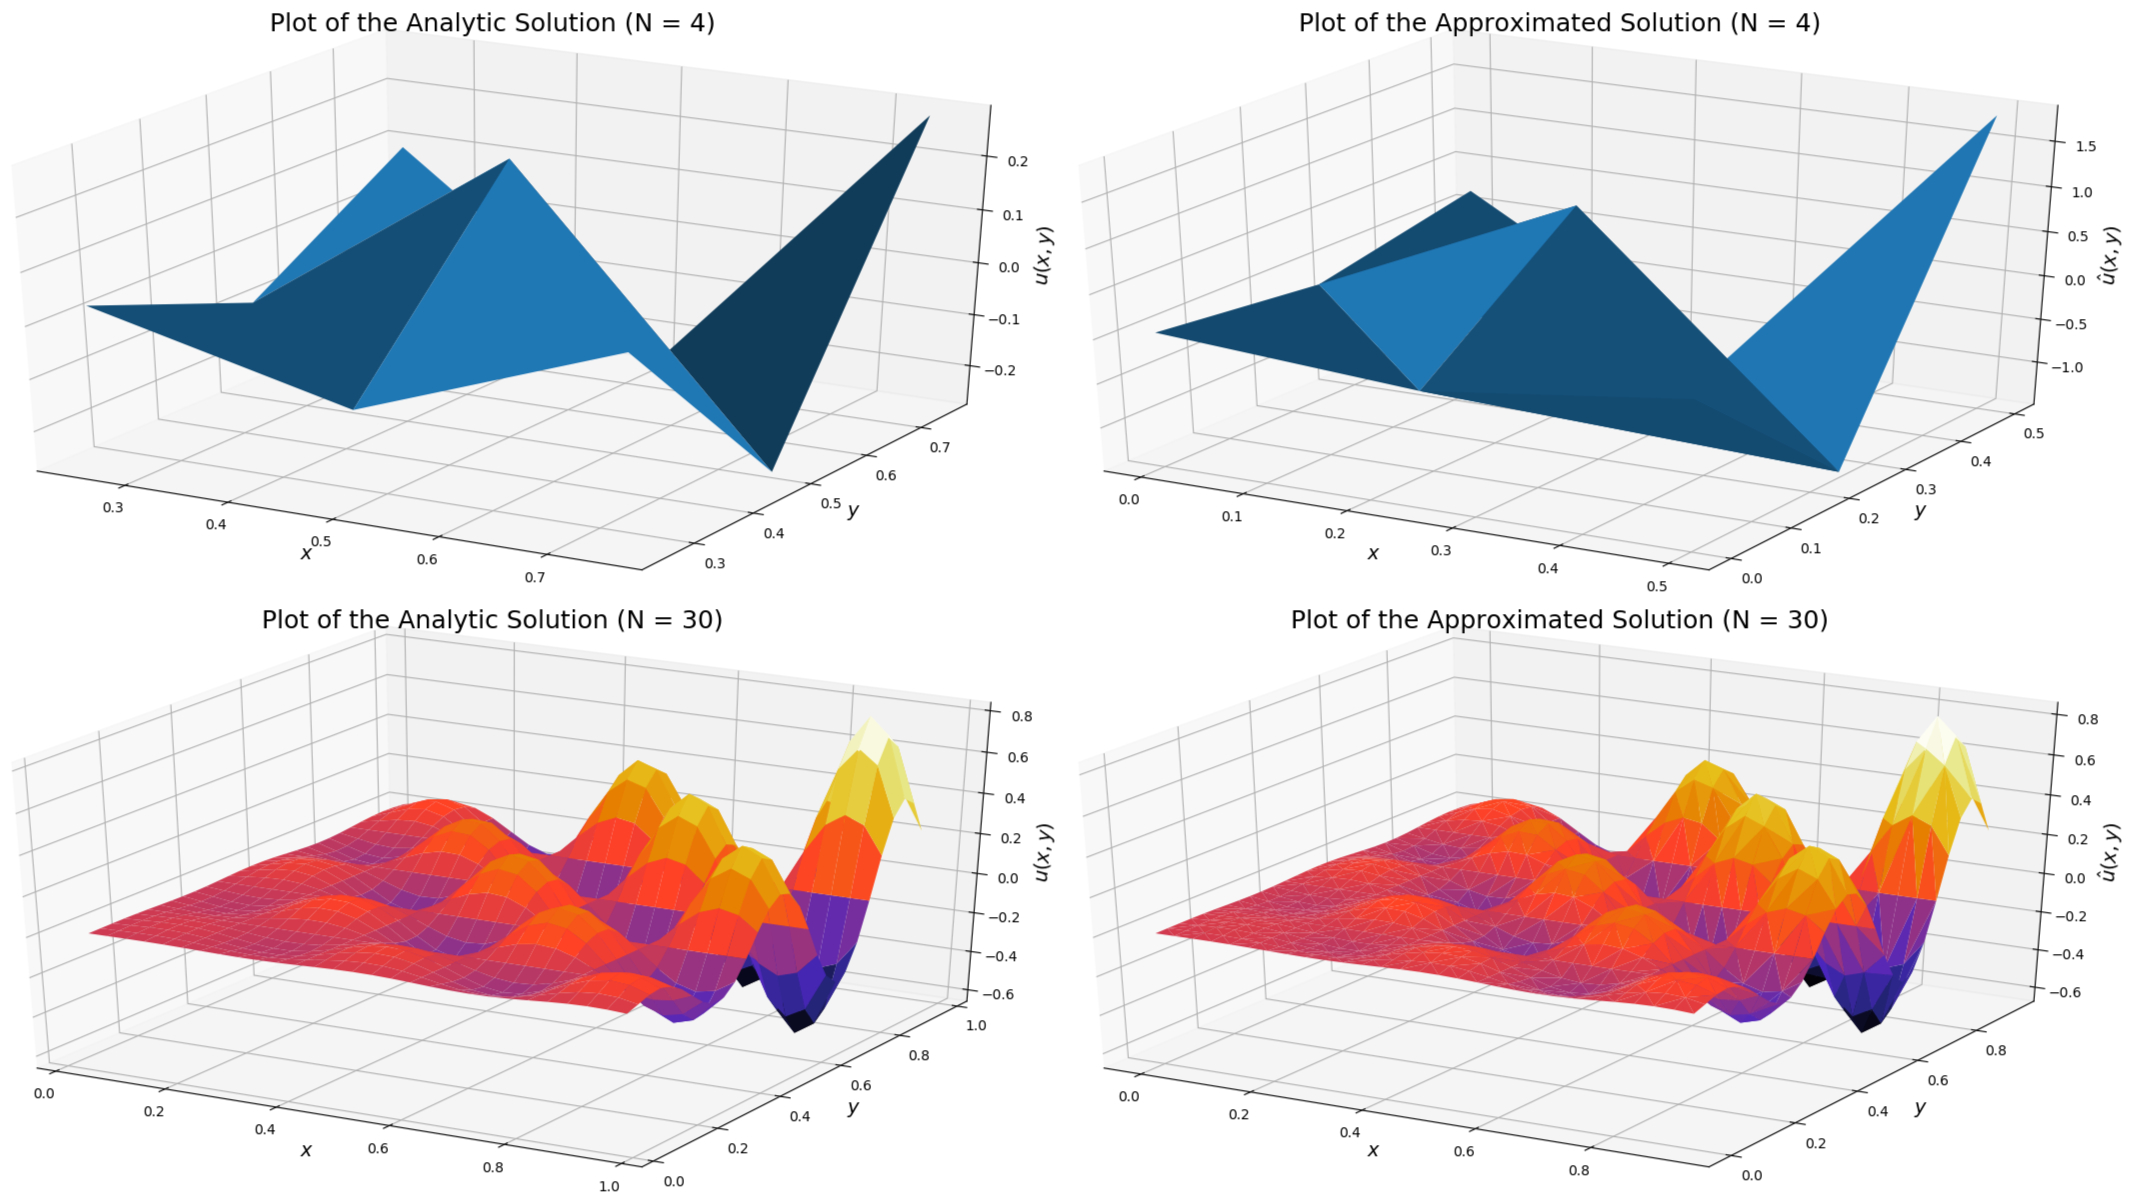
\includegraphics[width=\linewidth]{graphics/plot.jpg}
	\caption{Condition of the Hilbert Matrix}
	\label{fig:plots}
\end{figure}
\bigskip

\section{Analysis of the Sparsity}

\begin{figure}[h]
	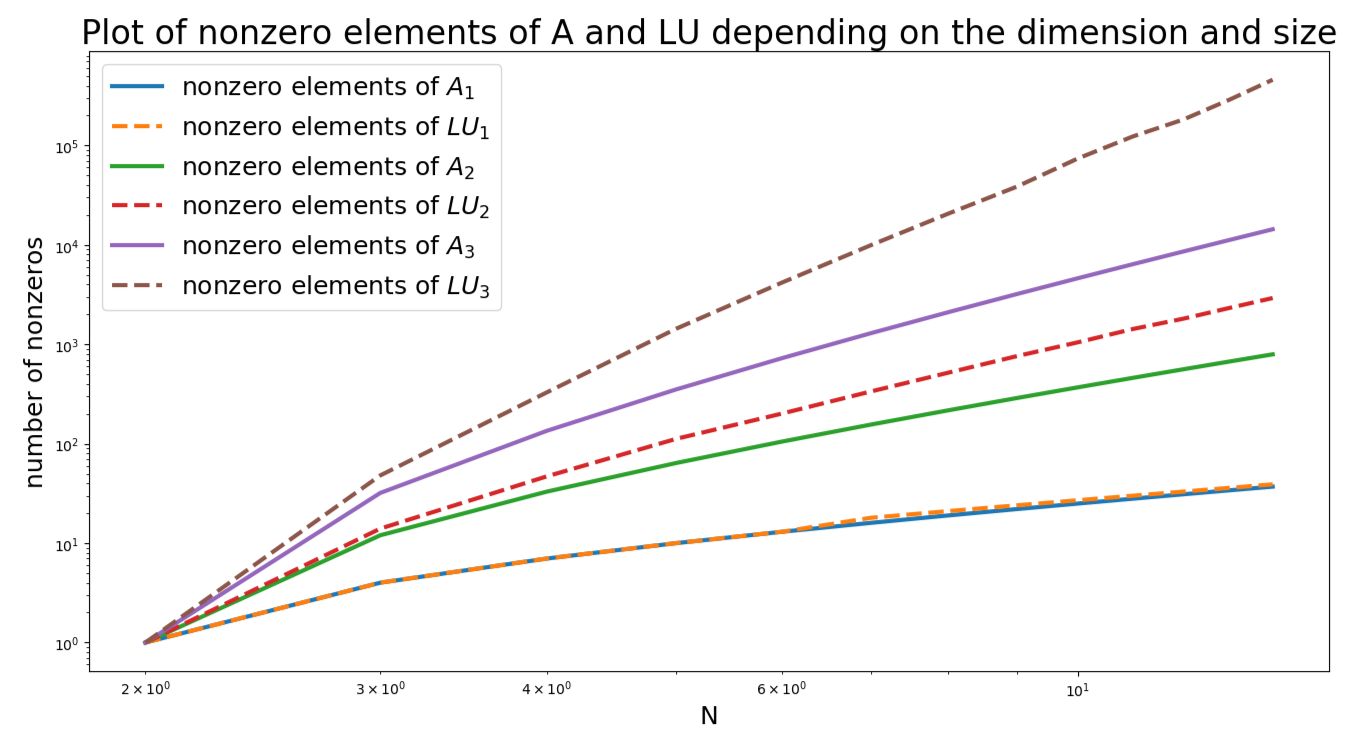
\includegraphics[width=\linewidth]{graphics/sparsity.png}
	\caption{Comparison of Nonzero Elements. The horizontal axis is the size of the matrix.}
	\label{fig:boat1}
\end{figure}

The sparsity structure of \(A^{(d)}\) is important because it allows us to save precious memory which in turn allows for larger computation. In this section, we want to compare the number of nonzero entries of \(A^{(d)}\) and its LU-decomposition. See figure \ref{fig:boat1} for the resulting plot.

With increasing size of \(A^{(d)}\) the amount of nonzero entries increases as well, and the LU-decomposition further adds more nonzeros to the problem. However, the speed by which the number of nonzero increases slows down. This means that larger matrices need more computation time, of course, but they are more sparse and hence less memory intensive.

\section{Conclusion}

In short, the Poisson's equation can be solved numerically via discretization of the domain, approximating the partial derivatives by finite differences and LU-decomposition. While the condition of the matrix \(A^{(d)}\) increases with its size, but this is counteracted by the fact that the numerical approximation of the Poisson's equation becomes more accurate as the number of grid points increases. Memory is also not a big issue thanks to the sparse structure of \(A^{(d)}\).

\begin{thebibliography}{9}
	\bibitem{protocol}
	Christian Parpart, Kei Thoma. 
	\textit{Numerical Approach to the Laplace Problem}. 
	2019.
\end{thebibliography}

\end{document}